 \documentclass[xcolor=dvipsnames,table]{beamer}

\usepackage{latexsym}
\usepackage[utf8]{inputenc}
\usepackage[brazil]{babel}
\usepackage{amssymb}
\usepackage{amsmath}
\usepackage{stmaryrd}
\usepackage{fancybox}
\usepackage{datetime}
\usepackage[T1]{fontenc}
\usepackage{graphicx}
\usepackage{graphics}
\usepackage{url}
\usepackage{algorithmic}
\usepackage{algorithm}
\usepackage{acronym}
\usepackage{array}



\newtheorem{definicao}{Definio}
\newcommand{\tab}{\hspace*{2em}}

\mode<presentation>
{
  \definecolor{colortexto}{RGB}{0,0,0}
 
  \setbeamertemplate{background canvas}[vertical shading][ bottom=white!10,top=white!10]
  \setbeamercolor{normal text}{fg=colortexto} 

  \usetheme{Warsaw}
}

\title{Tipos de Projetos em I\&E}  

\author{
  Esdras Lins Bispo Jr. \\ \url{bispojr@ufj.edu.br}
  } 
 \institute{
  Tópicos em Informática e Educação \\Bacharelado em Ciência da Computação}
\date{\textbf{06 de abril de 2026} }

\logo{
\includegraphics[width=1.5cm]{images/ufjJataiLogo.png}}

\begin{document}

	\begin{frame}
		\titlepage
	\end{frame}

	\AtBeginSection{
		\begin{frame}{Sumário}%[allowframebreaks]{Sumário}
    		\tableofcontents[currentsection]
    		%\tableofcontents[currentsection, hideothersubsections]
		\end{frame}
	}

	\begin{frame}{Plano de Aula}
		\tableofcontents
		%\tableofcontents[hideallsubsections]
	\end{frame}
	
	\section{Tipos de Projeto}

       \begin{frame}{Tipos de Projeto em I\&E}
           \begin{block}{Características}
               Cada tipo de projeto tem propósitos, escopos e resultados esperados que o marca de uma maneira singular.
           \end{block} \pause
           \begin{block}{Tipos mais comuns (universidade)}
               \begin{itemize}
                   \item Ensino
                   \item Pesquisa
                   \item Extensão
                   \item Inovação
               \end{itemize}
           \end{block}
       \end{frame}

       \subsection{Projetos de Ensino}

       \begin{frame}{Projetos de Ensino}
            \begin{block}{Propósito}
                Foco em aperfeiçoar a prática do ensino.
            \end{block} \pause
            \begin{block}{Escopo}
                Geralmente é restrito a uma única turma, ou instituição educacional.
            \end{block} \pause
            \begin{exampleblock}{Resultado Esperado}
                Mudança na prática (docente, discente, gestão, etc).
            \end{exampleblock}
           
       \end{frame}

        \begin{frame}{Exemplo: Projeto de Ensino}
            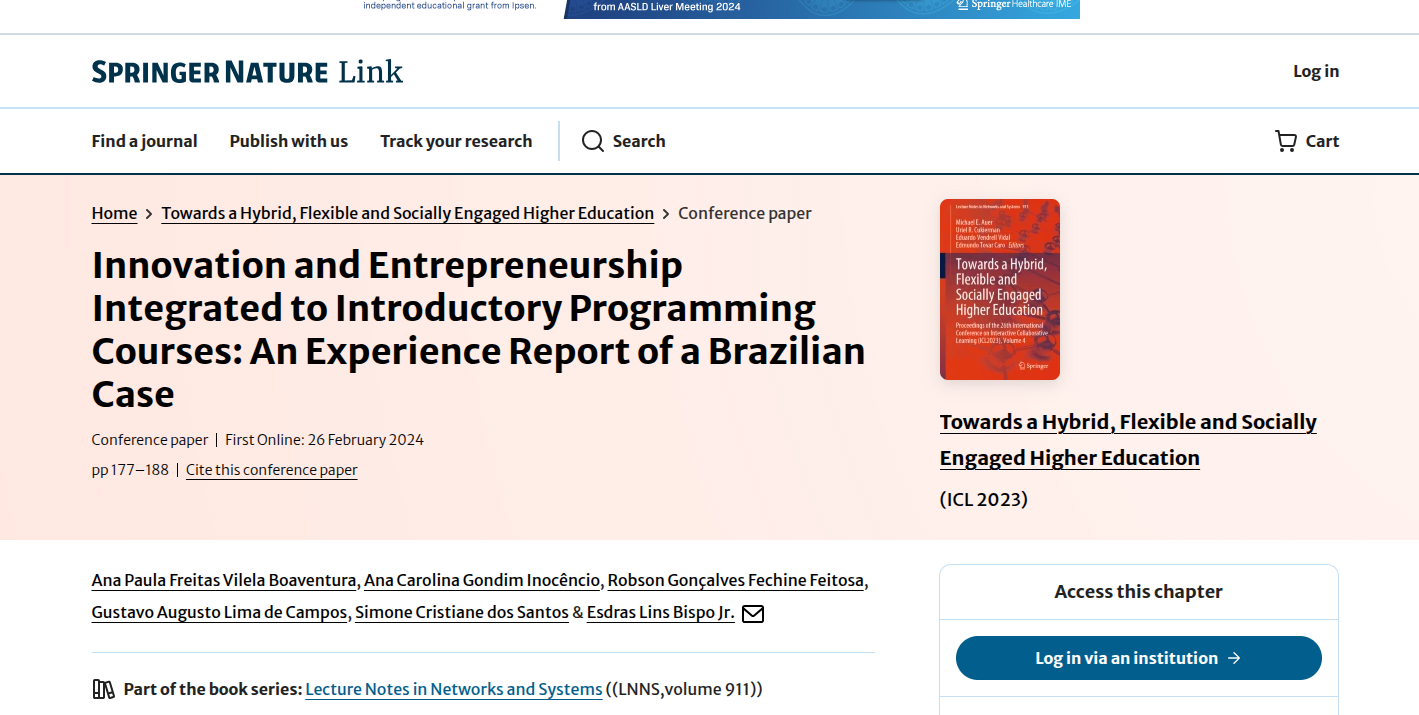
\includegraphics[width=\textwidth]{images/ensino.png}
            
        \end{frame}

        \subsection{Projetos de Pesquisa}

       \begin{frame}{Projetos de Pesquisa}
            \begin{block}{Propósito}
                Investigar sistematicamente novos conhecimentos por meio de métodos científicos.
            \end{block} \pause
            \begin{block}{Escopo}
                Geralmente delimitado por um objeto de pesquisa.
            \end{block} \pause
            \begin{exampleblock}{Resultado Esperado}
                Avanço do conhecimento em relação ao estado-da-arte de uma área.
            \end{exampleblock}
           
       \end{frame}

       \begin{frame}{Exemplo: Projeto de Pesquisa}
            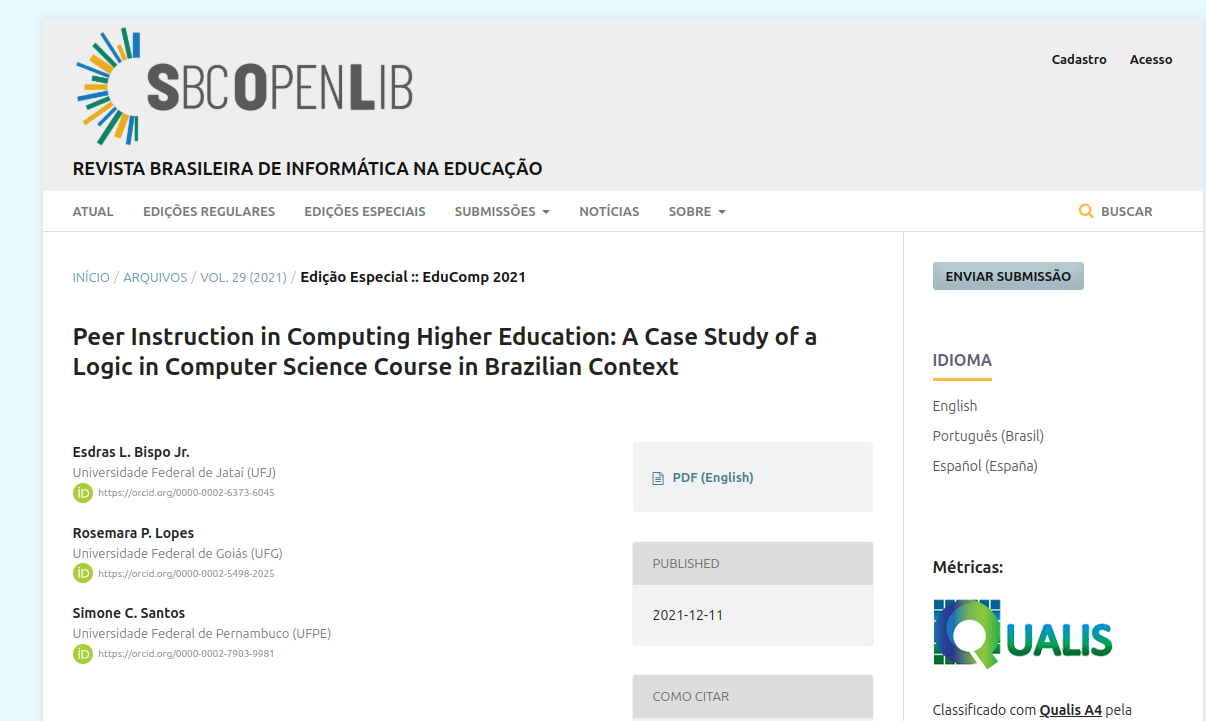
\includegraphics[width=\textwidth]{images/pesquisa.png}
            
        \end{frame}

        \subsection{Projetos de Extensão}

       \begin{frame}{Projetos de Extensão}
            \begin{block}{Propósito}
                Articulação da pesquisa e do ensino universitário junto à comunidade.
            \end{block} \pause
            \begin{block}{Escopo}
                Geralmente focado em espaços externos à universidade.
            \end{block} \pause
            \begin{exampleblock}{Resultado Esperado}
                Integração e Interação entre a universidade e a sociedade.
            \end{exampleblock}
           
       \end{frame}

       \begin{frame}{Exemplo: Projeto de Extensão}
            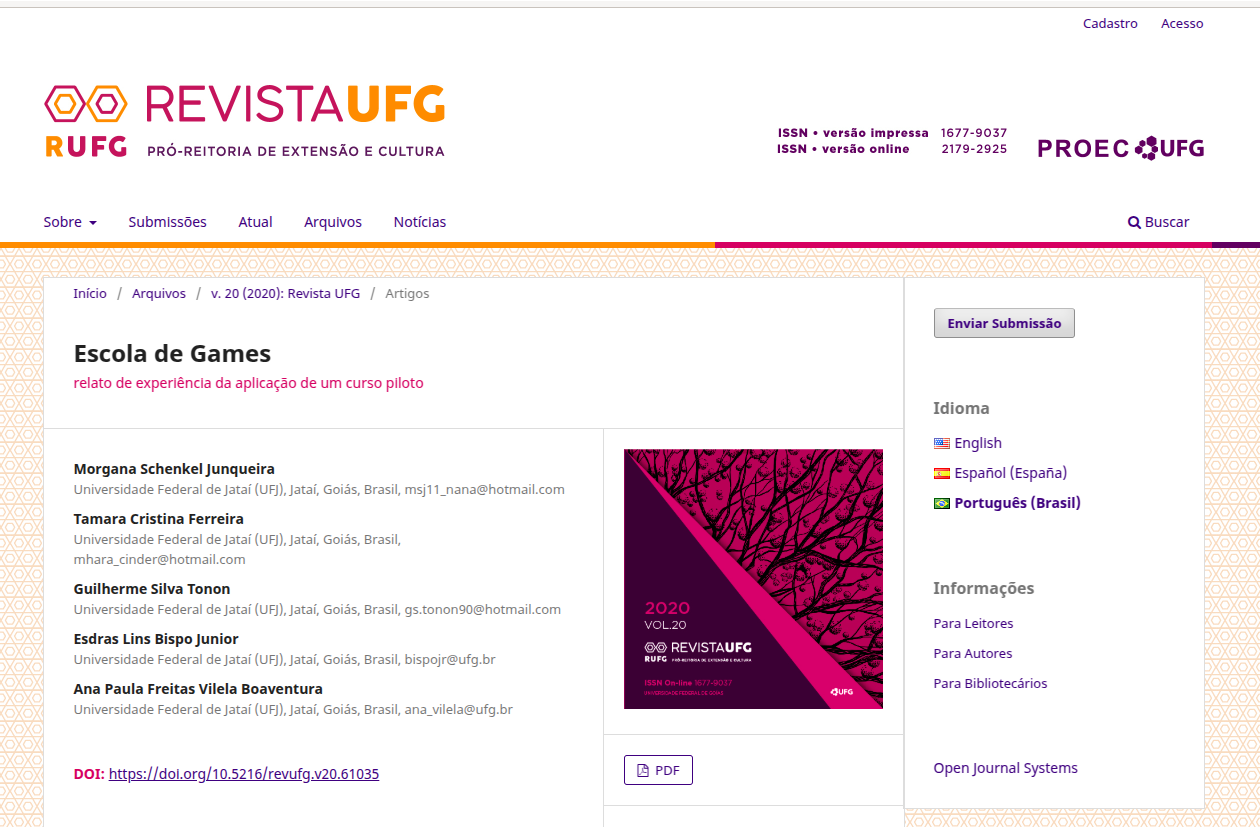
\includegraphics[width=\textwidth]{images/extensao.png}
            
        \end{frame}

        \subsection{Projetos de Inovação}

       \begin{frame}{Projetos de Inovação}
            \begin{block}{Propósito}
                Criação ou melhoria de novas ideias, produtos, serviços, ou métodos para um dado problema.
            \end{block} \pause
            \begin{block}{Escopo}
                Geralmento focados em contextos organizacionais.
            \end{block} \pause
            \begin{exampleblock}{Resultado Esperado}
                Oferecer valor, lucro ou soluções para determinados problemas.
            \end{exampleblock}
           
       \end{frame}

       \begin{frame}{Exemplo: Projeto de Inovação}
            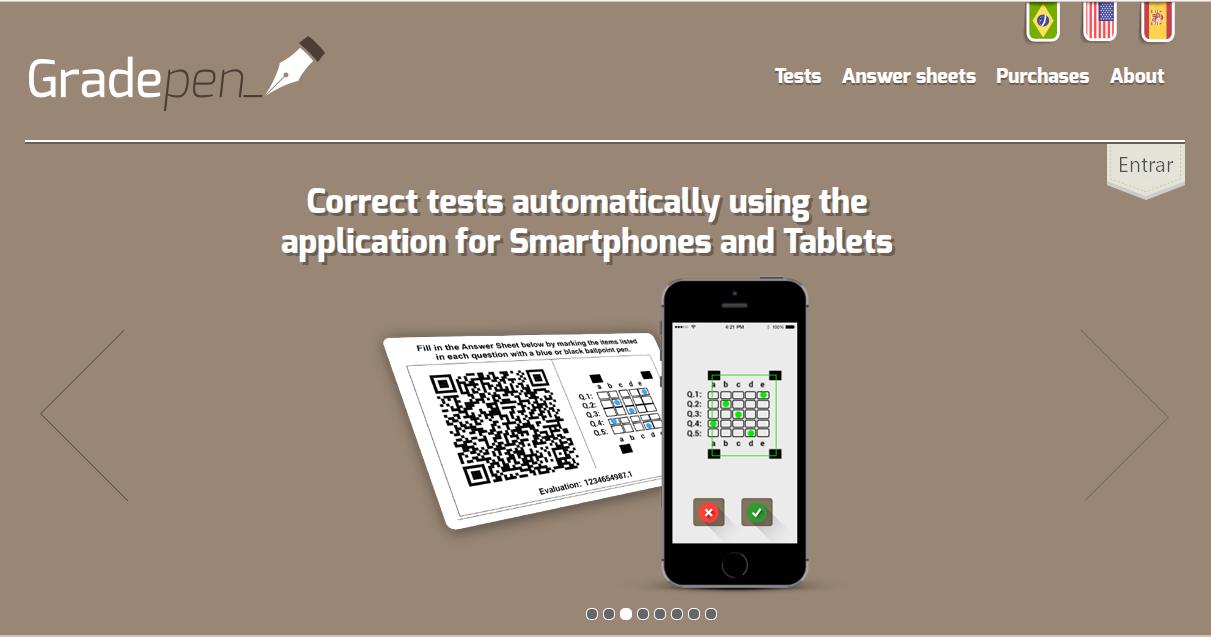
\includegraphics[width=\textwidth]{images/inovacao.png}
            
        \end{frame}
	
	\begin{frame}
		\titlepage
	\end{frame}
	
\end{document}